\documentclass[conference]{IEEEtran}



\usepackage{amsmath}
\usepackage{amssymb}
\usepackage{mathtools}
\usepackage{algorithmic}
%\usepackage{url}

% correct bad hyphenation here
\hyphenation{op-tical net-works semi-conduc-tor}


%%%%%%%%%%%%%% COMMANDS
\newcommand{\alg}{RQ-Learning\xspace}

\newcommand{\Rmodel}{\mathcal{R}}
\newcommand{\Pmodel}{\mathcal{P}}
\newcommand{\Rparams}[1][]{\boldsymbol{\omega}^{#1}}
\newcommand{\Rpspace}{\Omega}
\newcommand{\Rbasis}[1][]{\boldsymbol{\phi}\left({#1}\right)}
\newcommand{\Rmodelp}[1][\Rparams]{\mathcal{R}^{#1}}
\newcommand{\Rspace}[1][\dobj-1]{\Delta^{#1}}
\newcommand{\Simplex}[1][\dobj-1]{\mathbb{D}^{#1}}
\newcommand{\Rparamsdom}{\Theta^{*}}

\newcommand{\dsetexp}{\mathcal{D}}
\newcommand{\numdsetexp}{N}

\newcommand{\fe}[2][]{\boldsymbol{\mu}_{#2}\left(#1\right)}  %feature expectation
\newcommand{\feapx}{\widehat{\boldsymbol{\mu}}}                %approximate fe
\newcommand{\jval}[2][]{J_{#2}\left({#1}\right)}
\newcommand{\djval}[2][]{\Delta J_{#2}\left({#1}\right)}
\newcommand{\poly}{\mathcal{P}}
\newcommand{\radius}{r}
\newcommand{\acval}{\rho}
\newcommand{\targetset}{\mathbb{X}^{\epsilon}}

\newcommand{\dpolycut}{m}

\newcommand{\JvalMO}[2][\pi]{\boldsymbol{J}_{#2}\left(#1\right)}
%%%%%%%%%%%%%%%%%%%%%%%



%% math commands
\newcommand{\transpose}[1]{{#1}^\texttt{T}}
\DeclareMathOperator*{\argmax}{arg\,max}
\DeclareMathOperator*{\argmin}{arg\,min}
\DeclareMathOperator*{\EV}{\mathbb{E}}
\DeclareMathOperator*{\var}{\textbf{\texttt{Var}}}
\DeclareMathOperator*{\gradp}{\nabla_{\ppvect}}
\DeclareMathOperator*{\gradhp}{\nabla_{\hpvect}}

\newcommand{\norm}[2][\infty]{\left\|#2\right\|_{#1}}

\newcommand{\realspace}{\mathbb R}		% realspace

\newcommand{\statespace}{\mathcal X}		% state space
\newcommand{\actionspace}{\mathcal U}		% action space
\newcommand{\pmodel}{\mathcal P}		% transition function
\newcommand{\rmodel}{\mathcal R}		% reward function
\newcommand{\initD}{D}				% initial distribution

%% Vector and Matrix
\newcommand{\rvect}{\mathbf{R}}			% reward vector
\newcommand{\vvect}{\mathbf{V}}			% value function vector
\newcommand{\jvect}{\mathbf{J}}			% score vector
\newcommand{\gammavect}{\boldsymbol{\gamma}}	% gamma vector
\newcommand{\pmtx}{\mathbf{P}}			% transition matrix


\newcommand{\ppspace}{\Theta}
\newcommand{\pp}{\theta} 			% policy params
\newcommand{\ppvect}{\boldsymbol{\pp}}		% policy params vector (bold)
\newcommand{\vecop}{\text{vec }}
\newcommand{\sap}{\boldsymbol{z}}

\newcommand{\hpvect}{\boldsymbol \rho}
\newcommand{\hyperdist}{}

\newcommand{\Jvalapx}[1][\ppvect]{\widehat{J}\left({#1}\right)}
\newcommand{\Jval}[1][\ppvect]{J\left({#1}\right)}
\newcommand{\Jvalp}[2][\ppvect]{J_{#2}\left({#1}\right)}
\newcommand{\Mval}[1][\ppvect]{M\left({#1}\right)}
\newcommand{\Jvalvect}[1][\ppvect]{\jvect\left({#1}\right)}
\newcommand{\offJval}[1][\ppvect]{\mathcal{J}\left({#1}\right)}

\newcommand{\dstate}{n}
\newcommand{\daction}{m}
\newcommand{\dobj}{q}
\newcommand{\dpolicy}{d}

\newcommand{\numtraj}{N}

\newcommand{\horiz}{T}
\newcommand{\traj}{\tau}
\newcommand{\trajset}{\mathcal{T}}
\newcommand{\trajspace}{\mathbb{T}}
\newcommand{\trajlength}{T}
\newcommand{\trajR}{R}
\newcommand{\pdfunc}[1]{p\left(#1\right)}

\newcommand{\currstep}{t}	% index for current time step in GPOMDP derivations
\newcommand{\indxlogpi}{i}	% index for \sum \nabla log policy
\newcommand{\indxr}{j}		% index for \sum reward
\newcommand{\indxis}{w}		% index  for \prod importance sampling
\newcommand{\indxint}{k}	% index for \prod \int
\newcommand{\indxcomp}{k}	% index for \theta or gradient components
\newcommand{\indxcompr}{h}	% index for reward or gradient components

\newcommand{\Hessian}{\mathcal{H}}
\newcommand{\HJ}[1][\ppvect]{\Hessian_{\ppvect}\jvect({#1})}
\newcommand{\HJhat}[1][\ppvect]{\widehat{\Hessian}_{\ppvect}\jvect({#1})}
\newcommand{\HJREF}[1][\ppvect]{\widehat{\Hessian}_{\ppvect}^{RF}\jvect({#1})}
\newcommand{\HJGP}[1][\ppvect]{\widehat{\Hessian}_{\ppvect}^{GP}\jvect({#1})}
\newcommand{\glp}[1][]{\nabla_{\ppvect} \log \pi_{\ppvect}(a_{#1}|s_{#1})}
\newcommand{\hlp}[1][]{H_{\ppvect} \log \pi_{\ppvect}(a_{#1}|s_{#1})}

\newcommand{\EVV}[2][\ppvect \in \ppspace]{\EV_{#1}\left[{#2}\right]}
\newcommand{\EVVC}[3]{\EV_{\substack{#1}}\left[{#2}\middle|{#3}\right]}

\newcommand{\cMtx}[1][]{\mathcal{C}\left(#1\right)}
\newcommand{\basegrad}{b_{\nabla}}
\newcommand{\baseline}{b_\indxcomp}
\newcommand{\stepbaseline}{b^{(\currstep)}_\indxcomp}
\newcommand{\baseF}{F^{(\traj)}}
\newcommand{\baseG}{G_\indxcomp^{(\traj)}}
\newcommand{\stepbaseF}{F^{(\currstep)}}
\newcommand{\stepbaseG}{G_\indxcomp^{(\currstep)}}
\newcommand{\varr}[1][]{\textbf{\texttt{Var}}\left( {#1}\right)}

\newcommand{\pol}{\pi}
\newcommand{\polb}{\pi^{\mathcal{B}}}
\newcommand{\polt}{\pi^{\mathcal{T}}}

\newcommand{\qf}[1][^\pol]{Q#1}
\newcommand{\qffun}[2]{Q#1\left(#2\right)}		% value function with parenthesis

\newcommand{\mow}{\boldsymbol{\alpha}}
% \newcommand{\mow}{\Rparams}

\newcommand{\normv}{x}
\newcommand{\normpow}{y}
\newcommand{\ncost}[1][_{\normv}^{\normpow}]{\mathcal{C}{#1}}

\newcommand{\mdp}{\mathcal{M}}

\newcommand{\texsub}[1]{\textsc{\tiny #1}}


\usepackage{xspace}
\DeclareRobustCommand{\eg}{e.g.,\@\xspace}
\DeclareRobustCommand{\ie}{i.e.,\@\xspace}
\DeclareRobustCommand{\wrt}{w.r.t.\@\xspace}

%%
\newtheorem{Property}{Property}
\newtheorem{theorem}{Theorem}

% Q decomposition commands
\newcommand{\Rtilde}{\widetilde{R}}
\newcommand{\Qtilde}{\widetilde{Q}}


\begin{document}

\title{Reducing Uncertainty Propagation in Markov Decision Processes}


% author names and affiliations
% use a multiple column layout for up to three different
% affiliations
\author{\IEEEauthorblockN{Davide Tateo, Carlo D'Eramo, Alessandro Nuara, Marcello Restelli, Andrea Bonarini}
\IEEEauthorblockA{Department of Electronics, Information and Bioengineering\\
Politecnico Di Milano, Milano, Italy\\
Email: \{davide.tateo, carlo.deramo,  alessandro.nuara, marcello.restelli, andre.bonarini\}@polimi.it}
}

% make the title area
\maketitle

% As a general rule, do not put math, special symbols or citations
% in the abstract
\begin{abstract}
In many real-world problems stochasticity is a critical issue for the learning process. The sources of stochasticity come from the transition model, the explorative component of the policy or, even worse, from noisy observations of the reward function. For a finite number of samples, traditional Reinforcement Learning (RL) methods provide biased estimates of the action-value function leading to a poor estimation of the action-value function that is propagated to other action-values by the application of the Bellman operator. We propose an approach that significantly mitigates this issue avoiding the propagation of bad estimates of the action-value function.
\end{abstract}

% no keywords


% For peer review papers, you can put extra information on the cover
% page as needed:
% \ifCLASSOPTIONpeerreview
% \begin{center} \bfseries EDICS Category: 3-BBND \end{center}
% \fi
%
% For peerreview papers, this IEEEtran command inserts a page break and
% creates the second title. It will be ignored for other modes.
\IEEEpeerreviewmaketitle

\section{Introduction}
It is well known that a key issue of Reinforcement Learning (RL) problems is the accuracy of the estimation of the action-value with a limited number of samples. While most algorithms guarantee the convergence of the estimates to the optimal action-value, in practice the presence of stochastic components lead to poor performance. In fact, the majority of real-world problems have significant sources of stochasticity: the environment could have stochastic transition and this complicates the estimation of the effectiveness of an action; most of the times it is necessary to use stochastic policies to guarantee that all states are visited infinitely many times, that is required to guarantee the convergence of the algorithm; the policy could change during the learning process resulting in very different behaviors; the reward function is often corrupted by noisy observations and, in other cases, the reward function is stochastic itself. Moreover, it usually happens that some deterministic environments are partially observable and, thus, are perceived by the agent as stochastic decision processes (e.g. Blackjack).

Since Monte-Carlo estimates of action-values are affected by high variance of the returns, the most successful RL algorithms are based on bootstrapping (e.g. Q-Learning \cite{watkins1992q}), that trades off the variance of the estimation with a consistent but biased estimator. However with a finite number of samples the bias of the estimation could be significantly relevant when propagating the action-values to the next state and, recursively, it propagates to all the other states. Recent works tried to deal with this issue, in particular focusing on the estimation of the maximum expected value. 
%It is well known \cite{smith2006optimizer, van2004rational} that the maximum operator (used in the Q-Learning update) is positively biased, thus it overestimates the optimal action-value. In highly stochastic environments, this overestimation leads to unstable learning and poor convergence rates. To avoid the presence of the positive bias, the Double Q-Learning algorithm \cite{van2010double} has been proposed. This algorithm uses the double estimator \cite{van2013estimating} that provides a negatively biased estimation of the action-values (i.e. it underestimates the optimal action-value) and this improves the performance when stochasticity is an issue. Another recently proposed approach is the Weighted Q-Learning \cite{d2016estimating} that, computing a weighted average of the action-value functions estimates, balances between underestimation and overestimation. 
It is well known \cite{smith2006optimizer, van2004rational} that the maximum operator (used in the Q-Learning update equation) is positively biased, thus it overestimates the optimal action-value. In highly stochastic environments, this overestimation leads to unstable learning and poor convergence rates. In order to avoid this issue, the Double Q-Learning algorithm \cite{van2010double} has been proposed. This algorithm uses the double estimator \cite{van2013estimating} to compute the maximum in the updating formula of the Q-function. Providing a negatively biased estimation this value (i.e. it underestimates the optimal action-value),this approach can improve the performance especially in noisy environments.
Another recently proposed approach is the Weighted Q-Learning \cite{d2016estimating} that, computing a weighted average of the action-value functions estimates, balances between underestimation and overestimation. 

However, the correlation between bias of the estimation and performance is still unclear; indeed, as also shown in the empirical section of this paper, Speedy Q-Learning algorithm \cite{NIPS2011_4251} has very good performance despite its extremely poor estimation of the action-value. This is due to the fact that most of the policies are not dependent on the accuracy of the action-values, but instead they rely on their ordering. Starting from this considerations, we try to address this problem from another point of view. Indeed, we do not focus on the estimation of the maximum expected value, but we care about avoiding the propagation of uncertain action-value estimates. (DA CAMBIARE)In fact, we propose this work starting from the consideration that it is not relevant whether the approximations of the point estimates of the maximum expected value are good or not, but how these information is propagated to the other states. Our idea is to propagate the information about the value of the best action only when there is sufficiently certainty about the estimation.
In fact, we propose this work starting

The interesting aspect of this approach is that it is possible to use any maximum expected value estimator and, moreover, it can be easily extended in an on-policy scenario. Since we believe that in our approach the choice of the estimator is not a relevant issue, we choose the maximum operator as it is the simplest one.

\section{Preliminaries}
---TODO preso dal mio paper, va parafrasato, solo modifiche minori--
A Markov Decision Process (MDP) is defined by $\mathcal{M} = \langle \statespace,\actionspace,\Pmodel,\gamma,\Rmodel, D\rangle$, where $\statespace$ is the state space, $\actionspace$ is the action space, $\Pmodel$ is a Markovian transition model where $\Pmodel(x'|x,u)$ defines the transition density between state $x$ and $x'$ under action $u$, $\gamma\in[0,1)$ is the discount factor, $\Rmodel(r|x, u, x')$ defines the distribution of the reward, and $D$ is the distribution of the initial state.
A stochastic policy is defined by a density distribution $\pol(\cdot|x)$ that specifies for each state $x$ the density distribution over the action space $\actionspace$.
---
Given a policy $\pol$, we define the action value function as:
\begin{align}
 Q^\pol(x,u)=\underset{\strut\mathclap{\substack{(x', u')\sim \\ \Pmodel(x'|x,u)\pol(u'|x')}}}{\mathbb{E}}\left[ r(x,u,x')+\gamma Q^\pol(x,u)(x',u')\right]
 \label{eq:qpol}
\end{align}

The optmimal policy $\pol*$ is the policy with the highest expected return in the MDP. It has been proven that the optimal policy can be always represented by a deterministic policy. The optmimal action velue function $Q^*(x, u)$ is the action-value function of the optmimal policy.
It has been shown that the optimal policy in any MDP can be always a deterministic policy that at each state chooses the action with the highest $Q^*(x, u)$ value.

Given that we can always write the optimal action-value function as:
\begin{align}
 Q^*(x,u)=\underset{\strut\mathclap{x'\sim \Pmodel(x'|x,u)}}{\mathbb{E}}\left[ r(x,u,x')+\gamma\max_{u'} Q^*(x',u')\right]
 \label{eq:qopt}
\end{align}

As the expected value is a linear operator, we can always write \ref{eq:qopt} as:
\begin{align}
 Q^*(x,u)=\underset{\strut\mathclap{x'\sim \Pmodel(x'|x,u)}}{\mathbb{E}}\left[ r(x,u,x')\right]+\underset{\strut\mathclap{x'\sim \Pmodel(x'|x,u)}}{\gamma\mathbb{E}}\left[ \max_{u'} Q^*(x',u')\right]
 \label{eq:qdec}
\end{align}

We now introduce two functions, $\Rtilde$ and $\Qtilde$, defined as:
\begin{align}
 \Rtilde(x,u)&=\underset{\strut\mathclap{x'\sim \Pmodel(x'|x,u)}}{\mathbb{E}}\left[ r(x,u,x')\right] \nonumber\ \\
 \Qtilde(x,u)&=\underset{\strut\mathclap{x'\sim \Pmodel(x'|x,u)}}{\mathbb{E}}\left[\max_{u'} Q^*(x',u')\right]
 \label{eq:rqtilde}
\end{align}

We can give an interpretation of this two functions. $\Rtilde(x,u)$ is the expected immediate reward of the action $u$ in the state $x$. $\Qtilde(x,u)$ is the expected discounted return of the states reached after performing action $u$ in state $x$, i.e. the expected gain of the reached state.

We can now write the optimal value function as:
\begin{align}
 Q^*(x,u)=\Rtilde(x,u)+\gamma\Qtilde(x,u)
 \label{eq:qdecrqtilde}
\end{align}

Our approach shift the focus of the RL task from finding a good estimator for the optimal action-value function, to the task of finding good estimators for the $\Rtilde$ and $\Qtilde$ functions. The main motivation is that the sources of uncertainty of the two components of the action-value function are different: the $\Rtilde$ function only depends on the transition and reward models, while $\Qtilde$ also depends on the optmimal policy.

\section{The Proposed Method}

In the following section we will derive our method from \ref{eq:qdecrqtilde}. We will propose the general schema, using the maximum estimator and we will show the relations with the standard Q learning update.

\subsection{Decomposition of the TD Error}

Standard Q-Learning algorithm computes the temporal difference error given the tuple $(x,u,r,x')$ w.r.t. the current action-value estimates, and then updates such estimate proprotionally to the error. The amount of correction in the direction of the new sample is measured by the learning rate: if the learning rate is 1, the new sample substitutes the old estimate, if the learning rate is close to 0, the new sample is discarded, and the old estimate is kept unchanged. 
As shown in \ref{eq:qdecrqtilde} the action-value function could be decomposed in two different components. Our method is based on the idea to give separate estimates for this two components,
Instead of computing a TD error, we compute the error w.r.t. each component of the action-value function:

\begin{align}
\Rtilde(x,u) & \leftarrow\tilde{R}(x,u)+\alpha(R(x,u,x')-\Rtilde(x,u)) \label{eq:rtilupdedate}\\
\Qtilde(x,u) & \leftarrow\tilde{Q}(x,u)+\beta(\max_{u'}Q(x',u')-\Qtilde(x,u))
\label{eq:qtildeupdate}
\end{align}

Separating the two components of the value function can be useful, as the two components has inherently different sources of stochasticity. Moreover, the information stored in $\Rtilde$ is local to each state-action pair, and doesn't contain the uncertainty of the estimation of others states. The information stored in $\Qtilde$ instead depends only on the action-value function of the states that could be reached after performing the action $u$ in the state $x$, which, depends, recursively, on the others action-value functions. It is clear that the propagation of uncertain values only affects the $\Qtilde$ component.
As the actual action value function is the sum of the two estimates, we can write an equivalent update for the Q function:

\begin{align}
Q(x,u) & \leftarrow\tilde{R}(x,u)+\alpha(R(x,u,x')-\tilde{R}(x,u)) \nonumber\\
 & +\gamma\left(\tilde{Q}(x,u)+\beta(\max_{u'}Q(x',u')-\tilde{Q}(x,u))\right) \nonumber\\
 & =Q(x,u)+\alpha(R(x,u,x')-\tilde{R}(x,u)) \nonumber\\
 & +\gamma\beta(\max_{u'}Q(x',u')-\tilde{Q}(x,u))
 \label{eq:cumulativeupdate}
\end{align}

notice that this update cannot be used in practice in the algorithm, as it is not keeping the current values of the single components. However \ref{eq:cumulativeupdate} is useful to analyze the relations to standard Q-Learning algorithm.

\subsection{Analysis of the Decomposed Update}
We will discuss the relationship of our method with standard temporal difference methods. Let $t$ be the learning step. As a first step of our analysis we can consider the simplest case $\alpha(t)=\beta(t)$, $\forall t$.
by combining \ref{eq:cumulativeupdate} and \ref{eq:qdecrqtilde} we obtain:
\begin{align}
Q(x,u) & \leftarrow Q(x,u)+\alpha(R(x,u,x')+\gamma\max_{u'}Q(x',u')\nonumber\\
 & -Q(x,u))
\end{align}
That is the classical Q-Learning update. 

We consider now the setting $\alpha(t)\geq\beta(t)>0$, $\forall t$. Let $\beta(t)=\delta(t)\alpha(t)$, we obtain:
\begin{align}
Q(x,u) & \leftarrow Q(x,u)+\alpha(R(x,u,x')+\gamma\delta \max_{u'}Q(x',u') \nonumber\\
 & -(\tilde{R}(x,u)+\gamma\delta\tilde{Q}(x,u))) \nonumber\\
 & =Q(x,u)+\alpha(R(x,u,x')+\gamma'\max_{u'}Q(x',u') \nonumber\\
 & -(\tilde{R}(x,u)+\gamma'\tilde{Q}(x,u))) \nonumber\\
 & =Q(x,u)+\alpha((R(x,u,x')+\gamma'\max_{u'}Q(x',u')) \nonumber\\
 & -Q'(x,u))
\end{align}
With $\gamma'=\gamma\delta$. Notiche that $Q'(x,u)$ is the current Q function, but computed with a different discount factor. If the condition above is satisfied, then, we can see our method as a variable discount factor learning. If we consider $\delta(t)$ that increase monotonically in the interval $[0,1]$, our method is increasing each step the effective horizon, starting from trying to solve a greedy miopyc problem, and moving towards the real one. This approach, it has been used in practice to solve infinite horizon problems when the discount factor approach to 1,~\cite{}.

Finally, we can observe that, if the reward function and the transition model are deterministic, we can fix $\alpha$ to the value 1, while considering only $\beta(t)=\delta(t)$,

\subsection{Variance dependent learning rate}
To have better performance on the estimation, we would like to weight the error of each sample w.r.t. the current estimate depending on how much we are sure about the current value of our estimate. We propose then a learning rate that depends on the variance of the current variable estimate.

First of all we need to compute the variance of each estimator. To perform such computation we have to made the assumption that the learning rates are independent from the data. We will, of course, violate this assumption, but it is needed in order to have a closed form for the variance of the estimator, that can be used in practice. We will suppose also that the samples $X_i$ are i.i.d., with mean $\mu$ and variance $\sigma^2$. Consider the general form of the estimator:

\begin{align}
 \widetilde{X}_{n+1} = (1-\alpha(t))\widetilde{X}_{n}+\alpha(t)*\widetilde{X}
\end{align}

We now compute the expected value and the variance of this estimator:
\begin{align}
 \mathbb{E}\left[\widetilde{X}_{n+1}\right]& = \mu\sum_i^n \alpha(i) \prod_{j=i+1}^{n} \left(1-\alpha(j)\right)\\
 \mathrm{Var}\left[\widetilde{X}_{n+1}\right]& = \sigma^2\sum_i^n \alpha(i)^2 \prod_{j=i+1}^{n} \left(1-\alpha(j)\right)^2 = \sigma^2\omega
\end{align}

With $\omega=\sum_i^n \alpha(i)^2 \prod_{j=i+1}^{n} \left(1-\alpha(j)\right)^2$. Notice also that we can use the sample covariance $S_{n-1}$ of the random variable $X$ to estimate the real covariance $\sigma^2$. It is possible to compute in an incremental way both the sample covariance, in the traditional way, and $\omega$:

\begin{align}
 \omega_{n+1}=(1-\alpha(n))^2\omega_n+\alpha(n)^2
\end{align}

A weak assumption of this model, is that the variables are identically distribuited. While this should be true for the reward function, if the MDP is stationary, this is not true for the Q function values, whose distribution is affected by the policy and by the others states current estimates. However, a good approximation, could be to consider a window lenght in which the distribution is approximatively stationary: using such approach, we can compute the variance of the process in a given time window, forgetting old values that can lead to a biased estimation of the current variance. While this approach is not formally correct, as the derivation of the variance estimates makes the assumption of i.i.d. variables, this approximation has in practice have very good results.

Finally, we can choose a learning rate that depends on the covariance. Let $\sigma_e^2(t)$ be an estimate of $\mathrm{Var}\left[\widetilde{X}_{t}\right]$. We propose the following learning rate for each component of the action-value function:

\begin{align}
 \alpha(t)=\dfrac{\sigma_e^2(t)}{\sigma_e^2(t)+\eta}
\end{align}

Where $\eta$ is the amount of the estimator variance for wich the learning rate is $0.5$. It can be seen as a soft treshold to tune the speed of the decrease of the learning rate w.r.t. the estimator variance.

If we consider the case $\beta(t)=\alpha(t)\delta(t)$, then we have tu use a different learning rate. As we want an increase of the discount factor faster than the decrease of the general learning rate, we can use an exponentialy increasing learning rate for the delta parameter:

\begin{align}
 \delta(t) = 1- e^{\frac{\sigma^2}{\eta}\log(0.5)}
\end{align}

Where $\eta$ has the same iterpretation of the previous scenario.


\subsection{Convergence Properties}

TODO -- chiedere anche a restelli. Non banale!


\section{Experimental Results}
In this section we comparred the performance of the \emph{QD-Learning} with the most performing state of the art approaches (\emph{Q-learning,  Double Q-learning, Weighted Q-learning, Speedy Q-learning}) in three different problems.
\subsection{Stochastic (Van Hasselt?) GridWorld}
\section{Experimental results}
 \begin{figure*}[t]
  \begin{minipage}{\textwidth}
  \centering
   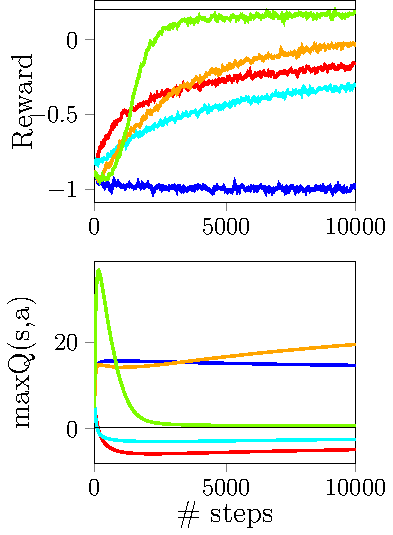
\includegraphics[width=.475\textwidth]{./imgs/gridHasselt/allAlgs1.pdf}
   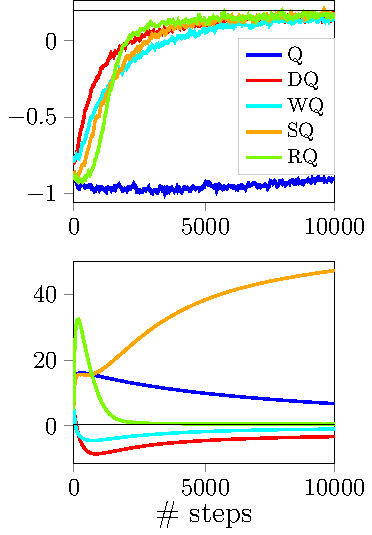
\includegraphics[width=.475\textwidth]{./imgs/gridHasselt/allAlgs08.pdf}\\
  \end{minipage}
   \caption{..}
   \label{F:hasselt_all}
 \end{figure*}
 \begin{figure*}[t]
  \begin{minipage}{\textwidth}
  \centering
   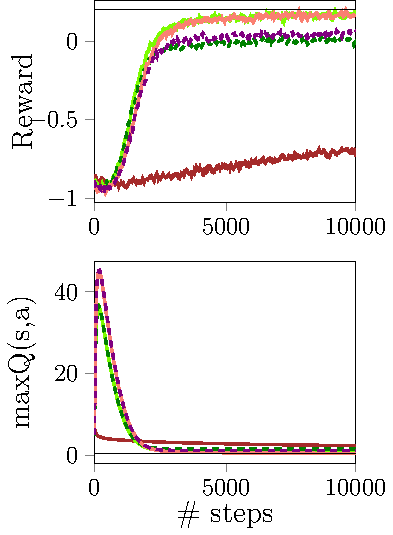
\includegraphics[width=.475\textwidth]{./imgs/gridHasselt/QDecs1.pdf}
   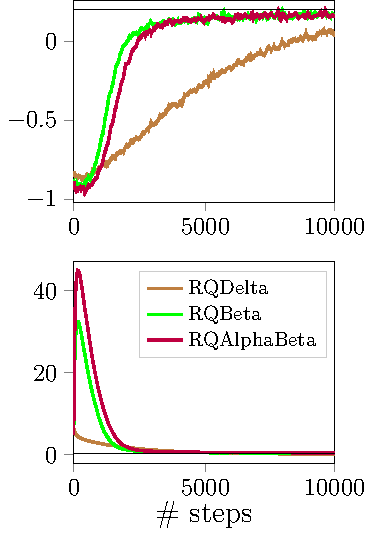
\includegraphics[width=.475\textwidth]{./imgs/gridHasselt/QDecs08.pdf}\\
  \end{minipage}
   \caption{..}
   \label{F:hasselt_all}
 \end{figure*}
 \begin{figure*}[t]
  \begin{minipage}{\columnwidth}
  \centering
   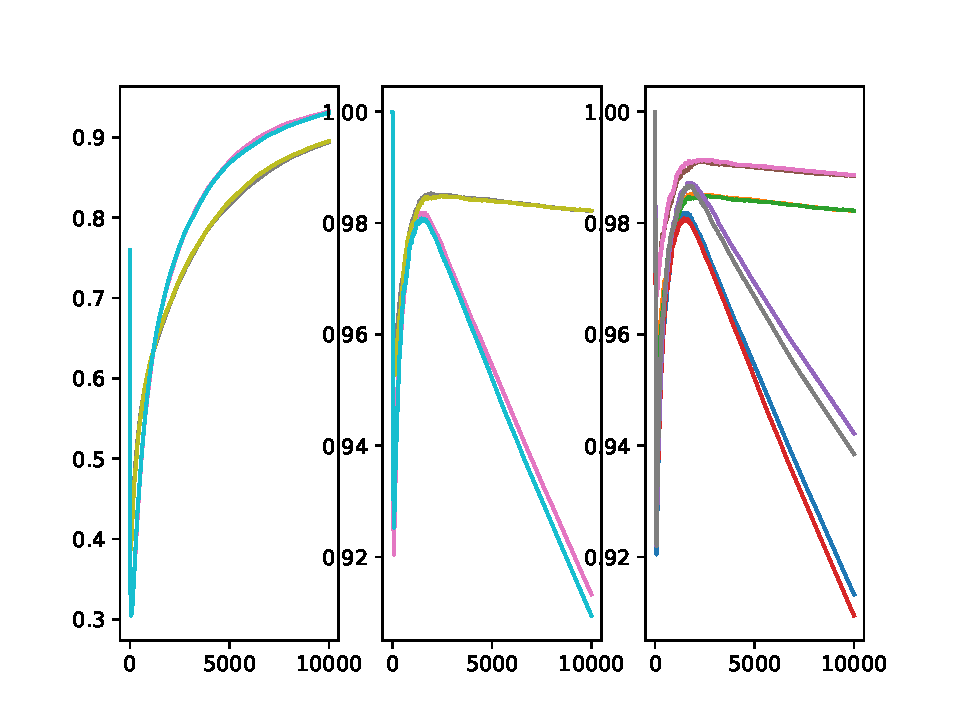
\includegraphics[width=\textwidth]{./imgs/gridHasselt/lrs.pdf}
  \end{minipage}
   \caption{..}
   \label{F:hasselt_all}
 \end{figure*}
We analyzed the performance in terms of average reward and Q-function estimation accuracy of the QD-Learning in a $3$x$3$ Gridworld with settings used in AAA. In this environment, the agent starts the episod from the lower-left position and has to reach the goal in the opposite position. The agent receives a Bernoullian reward -12 or +10 in all intermediate states and a deterministic reward +5 at the goal state. We used, for all algorithms, an	$\epsilon$-greedy policy $\epsilon = \frac{1}{\sqrt{n(s)}}$, where $n(s)$ is the number of  visits of the state $s$.


In Double Q-Learning we use two learning rates $\alpha_t^A(s, a) = \frac{1}{n_t^A(s, a)^{0.8}}$ and $\alpha_t^B(s, a) = \frac{1}{n_t^B(s, a)^{0.8}}$ where $n_t^A(s, a)$ and $n_t^B(s, a)$ are respectively the number of times when table A and table B are updated. 
The optimal average reward per step is $0.2$ and the maximum action-value function of the starting state is $5\gamma^4 - \sum_{k=0}^3 \gamma^k \approx 0.36$.
\subsection{Come si chiama Gridworld}

\subsection{Double Chain}

\section{Conclusion}


% trigger a \newpage just before the given reference
% number - used to balance the columns on the last page
% adjust value as needed - may need to be readjusted if
% the document is modified later
%\IEEEtriggeratref{8}
% The "triggered" command can be changed if desired:
%\IEEEtriggercmd{\enlargethispage{-5in}}

% references section

% can use a bibliography generated by BibTeX as a .bbl file
% BibTeX documentation can be easily obtained at:
% http://mirror.ctan.org/biblio/bibtex/contrib/doc/
% The IEEEtran BibTeX style support page is at:
% http://www.michaelshell.org/tex/ieeetran/bibtex/
\bibliographystyle{IEEEtran}
% argument is your BibTeX string definitions and bibliography database(s)
\bibliography{biblio}



% that's all folks
\end{document}


